\documentclass{ethz_report}
\usepackage{listings}
\usepackage{color}
\usepackage{caption}
\usepackage{subcaption}


\definecolor{codegreen}{rgb}{0,0.6,0}
\definecolor{codegray}{rgb}{0.5,0.5,0.5}
\definecolor{codepurple}{rgb}{0.58,0,0.82}
\definecolor{backcolour}{rgb}{1,1,1}

\lstdefinestyle{mystyle}{
    backgroundcolor=\color{backcolour},
    commentstyle=\color{codegreen},
    keywordstyle=\color{magenta},
    numberstyle=\tiny\color{codegray},
    stringstyle=\color{codepurple},
    basicstyle=\ttfamily,
    breakatwhitespace=false,
    breaklines=true,
    captionpos=b,
    keepspaces=true,
    numbers=left,
    numbersep=5pt,
    showspaces=false,
    showstringspaces=false,
    showtabs=false,
    tabsize=4,
    frame=lines
}
\lstset{style=mystyle}

\title{Exercise 7 - Structure from Motion}
\subject{Computer Vision}
\author{Alberto Montes}
\email{malberto@student.ethz.ch}
\date{\today}

\begin{document}
\maketitle

\section*{Feature extraction and initialization with epipolar geometry}

For the first task, first it was required to initialize the structure with two images (the first and last one) matching its features. First the SIFT features were extracted for both images and matched by the descriptors extracted. The resulting matching is on Figure~\ref{fig:sift_feat_matching}.

Then the 8-point RANSAC algorithm has been used to compute the inlier-set and then compute the essential matrix. This provide a better matching and can be seen on Figure~\ref{fig:init_inliers}.

\begin{figure}[H]
    \centering
    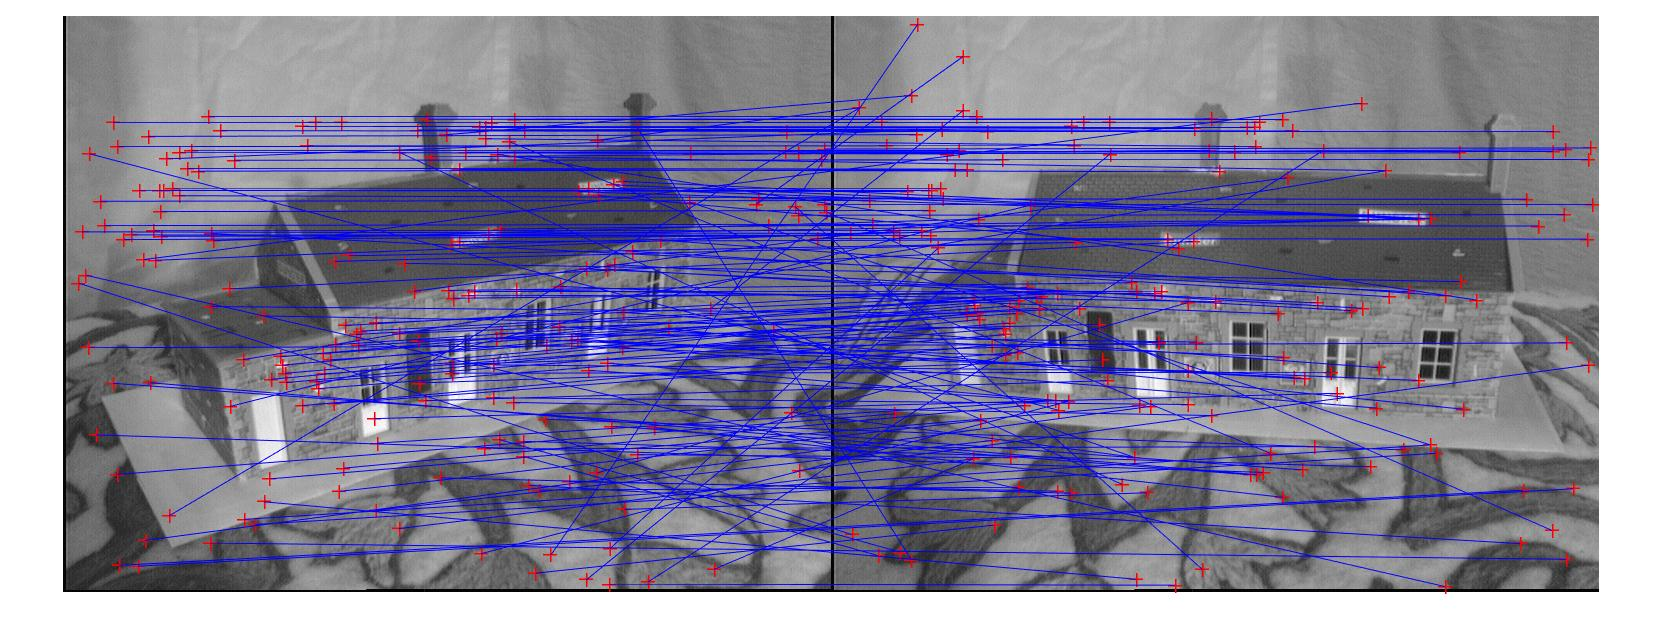
\includegraphics[width=1\linewidth]{images/ini_raw}
    \caption{SIFT features matching}
    \label{fig:sift_feat_matching}
\end{figure}

\begin{figure}[H]
    \centering
    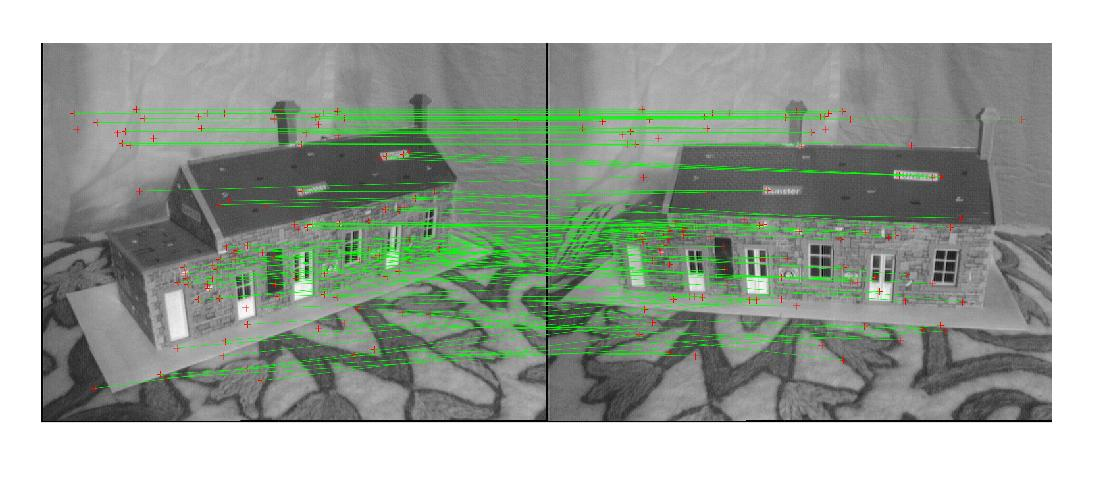
\includegraphics[width=1\linewidth]{images/ini_inliers}
    \caption{Inliers features matching using 8-point RANSAC algorithm}
    \label{fig:init_inliers}
\end{figure}

Then the image inliers points are calibrated using the $K$ matrix and decompose the Essential Matrix
to obtain the camera matrix. Finally the matched points are triangulated to obtain the 3D representation. The implementation is listed in the Listing~\ref{lst:code1}.

\lstinputlisting[language=MATLAB, caption=Compute essential matrix and projection matrices, firstline=35, lastline=52, label={lst:code1}]{../code/exercise8.m}

\section*{Triangulation and adding new views}

The next task has been to add a new triangulation from a new view. To do so, first it has been selected the descriptors of the first view which have projected in the linear triangulation. With this descriptors and the ones extracted to the new view, a feature matching has been performed. Now, having an initial correspondence between 3D points of the previous triangulation and the 2D points of the new view's features, a 6-point RANSAC algorithm is used to compute the projection matrix and the inliers points. The inliers matchings resulting from this algorithm at each of the views is plotted at Figure~\ref{fig:inliers_projection_matrix}.

\begin{figure}[h]
    \centering
    \begin{subfigure}[b]{.5\textwidth}
        \centering
        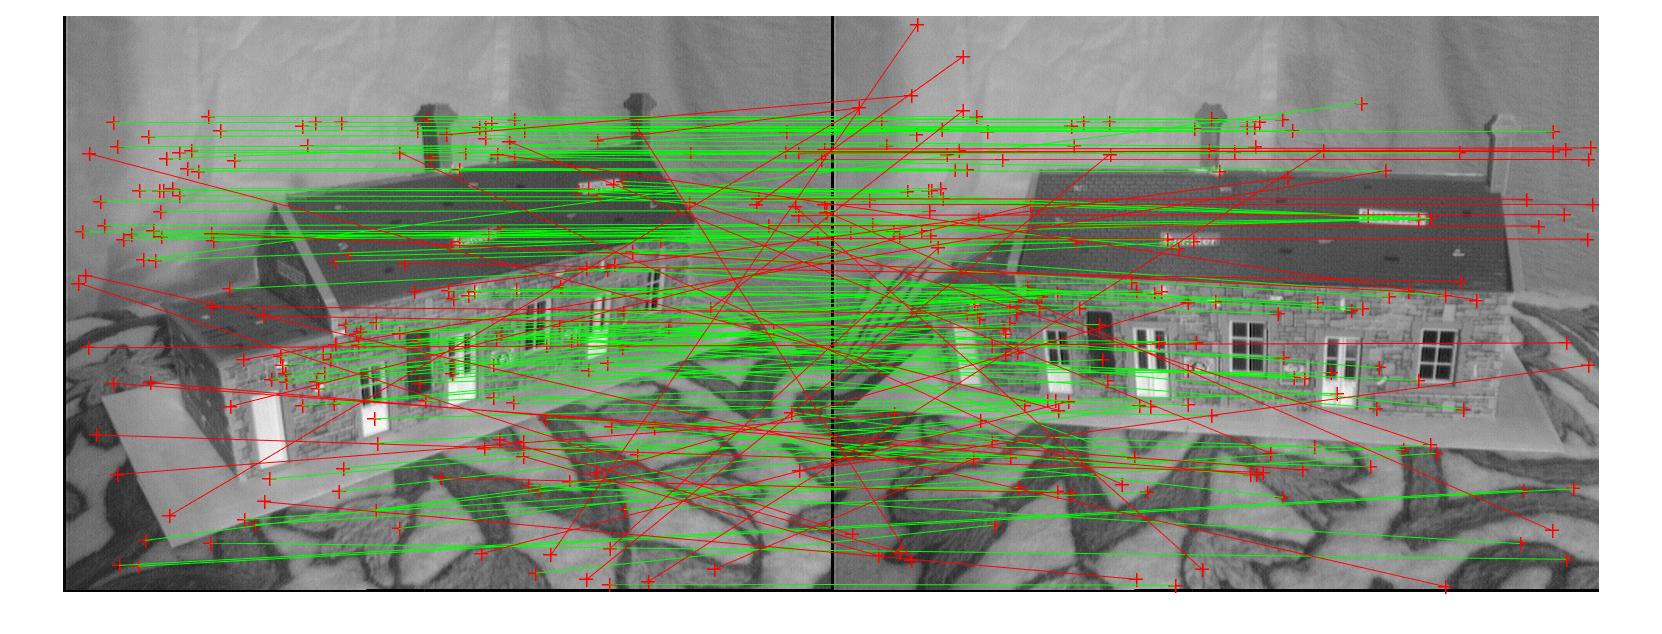
\includegraphics[width=1\linewidth]{images/ini_inliers_outliers_1}
        \caption{\texttt{house.000} $\leftrightarrow$ \texttt{house.001}}
    \end{subfigure}%
    \begin{subfigure}[b]{.5\textwidth}
        \centering
        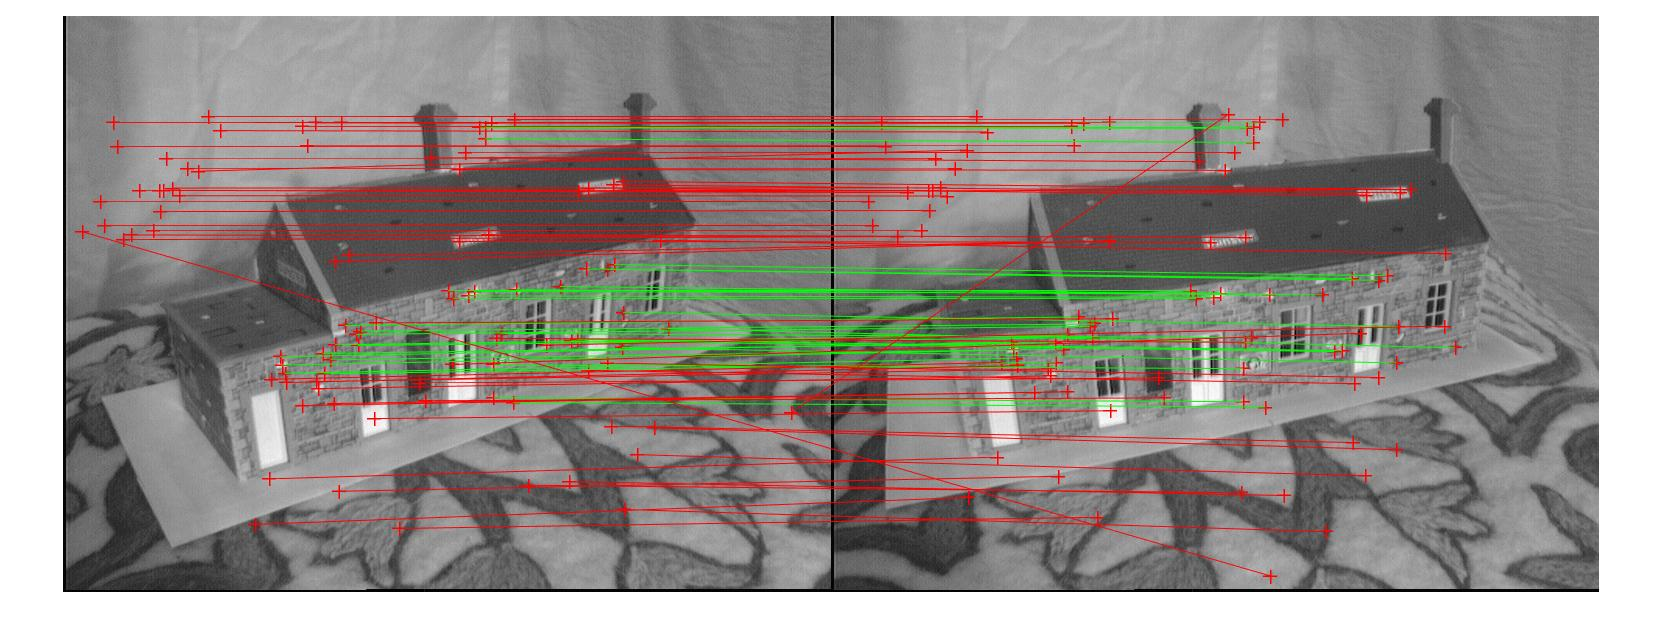
\includegraphics[width=1\linewidth]{images/ini_inliers_outliers_2}
        \caption{\texttt{house.000} $\leftrightarrow$ \texttt{house.002}}
    \end{subfigure}
    \begin{subfigure}[b]{.5\textwidth}
        \centering
        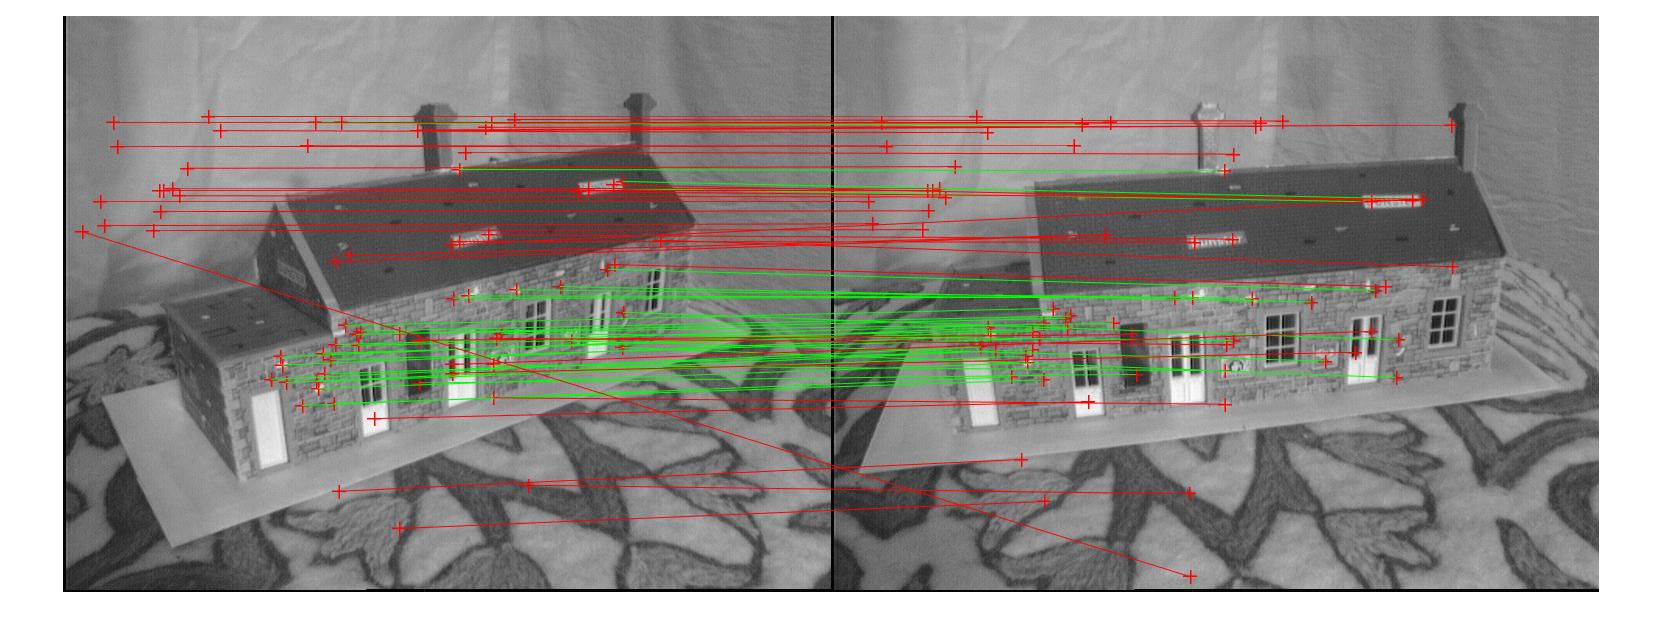
\includegraphics[width=1\linewidth]{images/ini_inliers_outliers_3}
        \caption{\texttt{house.000} $\leftrightarrow$ \texttt{house.003}}
    \end{subfigure}
    \caption{Inliers features matching using 6-point RANSAC algorithm to find the Projection Matrix}
    \label{fig:inliers_projection_matrix}
\end{figure}

The implemented code is shown in Listing~\ref{lst:code2} where all the steps are implemented with the given functions with the exercise statement.

\lstinputlisting[language=MATLAB, caption=Compute essential matrix and projection matrices for new views, firstline=54, lastline=74, label={lst:code2}]{../code/exercise8.m}

\section*{Plotting}

The final part of the exercise consist on triangulate all inlier matches from all the views in a 3D representation. On Figure~\ref{fig:3d_projection} there is the 3D plot of all the inlier points projected. On the plot can be observed how the number of red points (which correspond to the inlier features at the initialization) is much higher because than the rest of the views, as it was required to fit for each view the projection matrix using the RANSAC algorithm. Although, the projected points obtained look very consistent as can be observed a overlap between same features projections. Also the camera representation look to be correct as it plots the approximated locations where all the images where taken for this task.

\begin{figure}[h]
    \centering
    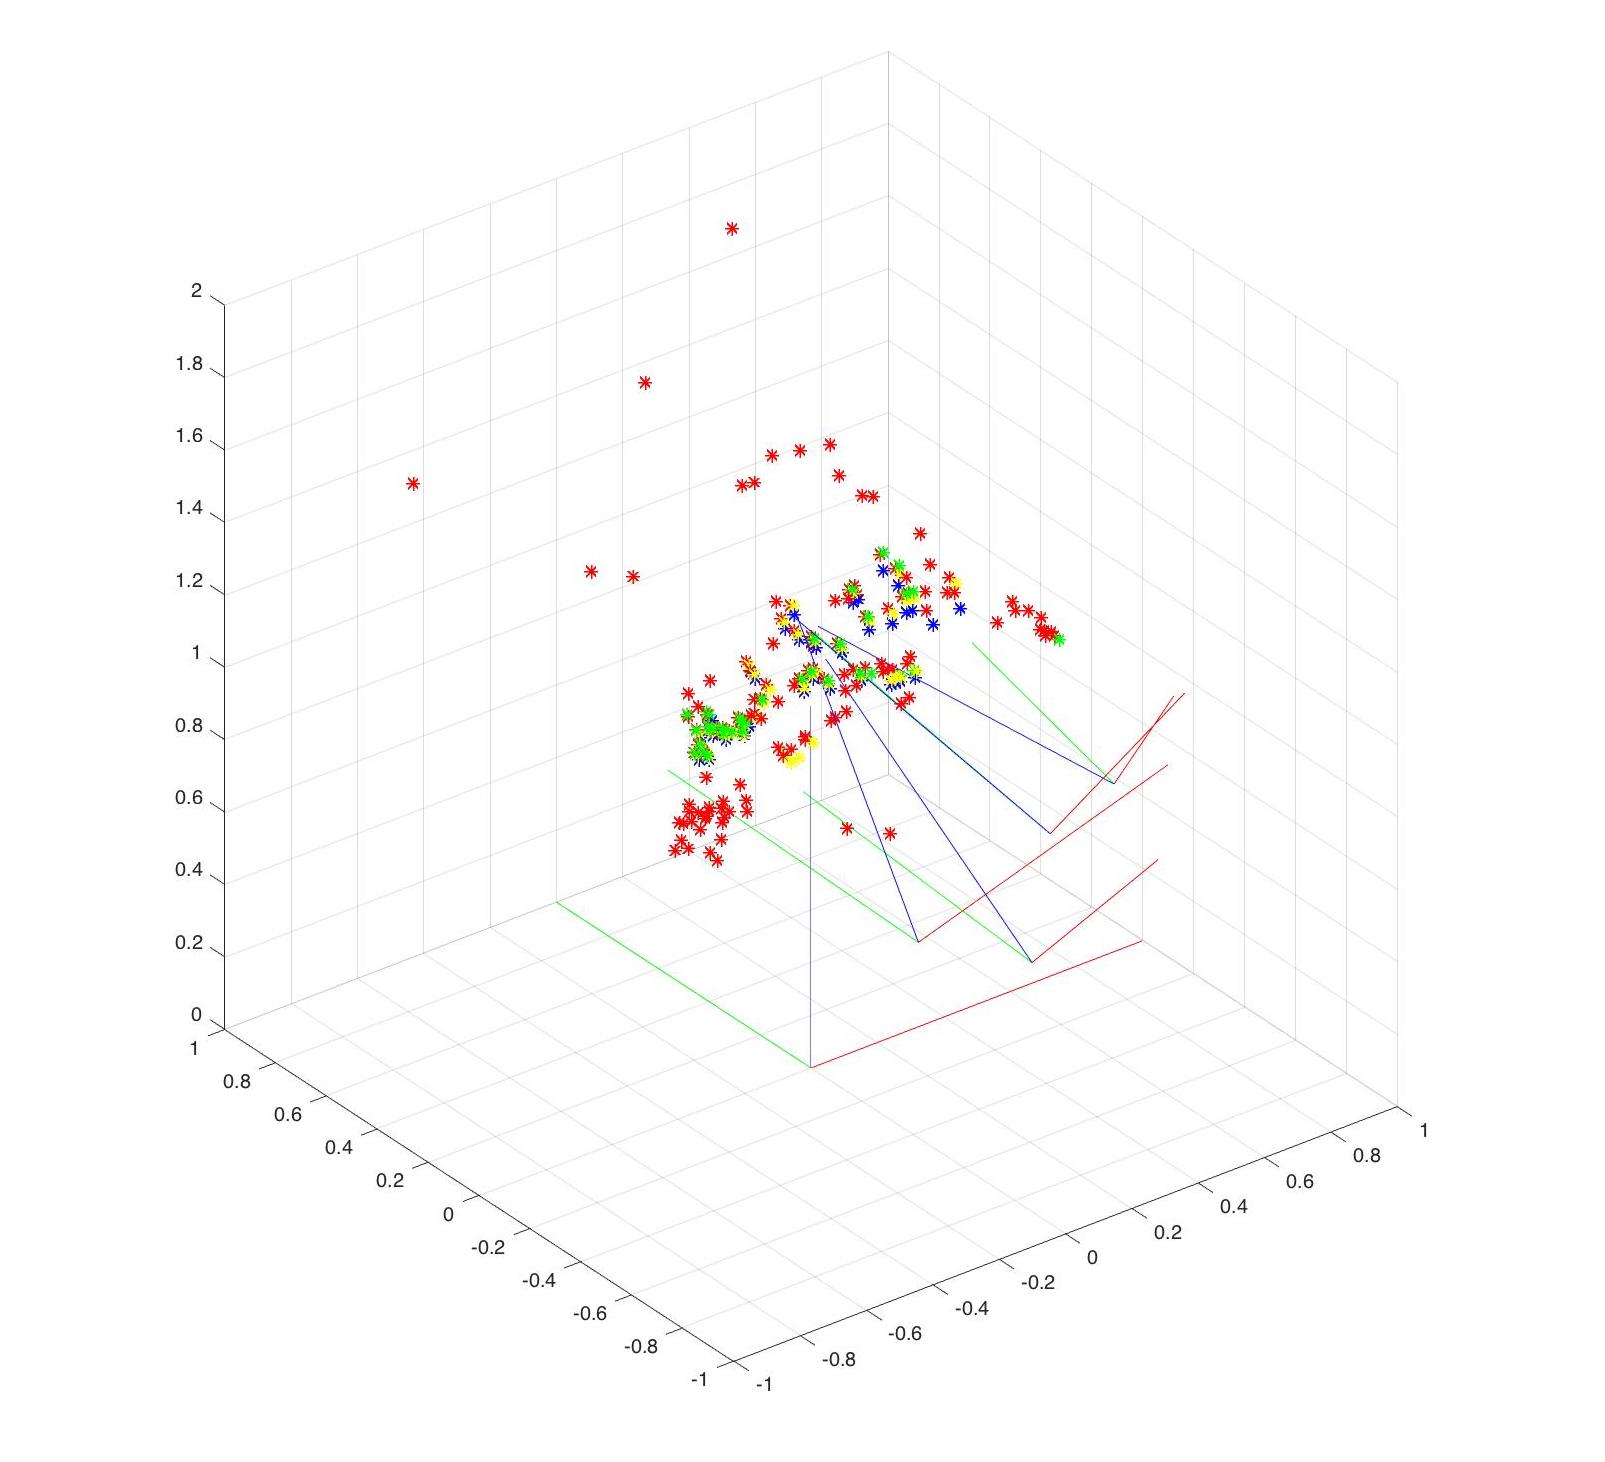
\includegraphics[width=1\linewidth]{images/points3d_projection}
    \caption{3D projection of all the inlier features.}
    \label{fig:3d_projection}
\end{figure}


\end{document}
